\documentclass[11pt,oneside]{article}
\usepackage{subfigure}
\usepackage{amsmath}
\usepackage{amssymb}
\usepackage{amsbsy}
\usepackage{mathpazo}
\usepackage{float}
\usepackage{braket}
\setlength {\marginparwidth }{3cm}
\usepackage{todonotes}
\usepackage[spanish]{babel}
\usepackage{graphicx}
\usepackage{listings}
\usepackage{color}
\usepackage{booktabs}
\usepackage{multirow}
\usepackage{ragged2e}
\usepackage{amsmath,blkarray,booktabs,bigstrut}
\usepackage[a4paper, left=2.5cm, right=2.5cm, top=2.5cm, bottom=2.5cm]{geometry}
\usepackage{hyperref}
\usepackage{colortbl}
\usepackage{xcolor}
\usepackage{enumitem}
\usepackage{tcolorbox}
\usepackage{todonotes}

\hypersetup{
    colorlinks=true,
    linkcolor=blue, % Color de los enlaces internos
    filecolor=magenta, % Color de los enlaces a archivos
    urlcolor=blue % Color de los enlaces a URLs
}

\floatstyle{ruled}
\restylefloat{table}

\usepackage{listings}
\usepackage{color}
\lstloadlanguages{csh}

\definecolor{red}{rgb}{0.6,0,0} 
\definecolor{blue}{rgb}{0,0,0.6}
\definecolor{green}{rgb}{0,0.8,0}
\definecolor{cyan}{rgb}{0.0,0.6,0.6}
\definecolor{white}{rgb}{1,1,1}

% Configuración global para todos los recuadros
\tcbset{
    colback=blue!3!white,     % Fondo
    colframe=blue!50!white,   % Borde 
    boxrule=0.5mm,            % Grosor del borde (opcionalmente más delgado)
    title=Información         % Título predeterminado
}

\lstset{
language=csh,
captionpos=b,      % Posición del caption (b: abajo, t: arriba)
basicstyle=\footnotesize\ttfamily,
% numbers=left,
% numberstyle=\tiny,
% numbersep=5pt,
tabsize=2,
extendedchars=true,
% breaklines=true,
% frame=b,
stringstyle=\color{red}\ttfamily,
showspaces=false,
showtabs=false,
% xleftmargin=17pt,
framexleftmargin=17pt,
% framexrightmargin=5pt,
framexbottommargin=4pt,
commentstyle=\color{green},
morecomment=[l]{//}, %use comment-line-style!
morecomment=[s]{/*}{*/}, %for multiline comments
showstringspaces=false,
morekeywords={ abstract, event, new, struct,
as, explicit, null, switch,
base, extern, object, this,
bool, false, operator, throw,
break, finally, out, true,
byte, fixed, override, try,
case, float, params, typeof,
catch, for, private, uint,
char, foreach, protected, ulong,
checked, goto, public, unchecked,
class, if, readonly, unsafe,
const, implicit, ref, ushort,
continue, in, return, using,
decimal, int, sbyte, virtual,
default, interface, sealed, volatile,
delegate, internal, short, void,
do, is, sizeof, while,
double, lock, stackalloc,
else, long, static, get,
enum, namespace, string},
keywordstyle=\color{blue},
identifierstyle=\color{black},
backgroundcolor=\color{white},
inputencoding=utf8,
    literate=%
    {á}{{\'a}}1
    {é}{{\'e}}1
    {í}{{\'i}}1
    {ó}{{\'o}}1
    {ú}{{\'u}}1
    {Á}{{\'A}}1
    {É}{{\'E}}1
    {Í}{{\'I}}1
    {Ó}{{\'O}}1
    {Ú}{{\'U}}1
    {ñ}{{\~n}}1
    {Ñ}{{\~N}}1
    {¡}{{\textexclamdown}}1
    {¿}{{\textquestiondown}}1
}

% Definir tipos personalizados en cian
\lstset{
    classoffset=1,
    morekeywords={
    Program, Console, List, StringBuilder, Array,
    TypeOfTriangle, DayOfWeek,
    NotImplementedException, DivideByZeroException, ArgumentException, 
    ChessPiece,
    BigInt, Fraction, Poly, Set, Book, Genre},
    keywordstyle=\color{cyan},
    classoffset=0,
}

\renewcommand{\lstlistingname}{Figura} % Cambia el prefijo de lstlisting a "Figura"

% Define la variable para controlar la visibilidad de las respuestas
\newif\ifshowanswers

% Define la variable que representa el curso
\def\academicyear{2024 - 2025}

% \showanswerstrue  % Comenta esta línea para ocultar las respuestas

\begin{document}
    \begin{center}
    \begin{large}
    Cp 9 - Recursividad\\
    Curso \academicyear\\
    \end{large}
    % \begin{figure}[h]
    % 	\centering
    % 	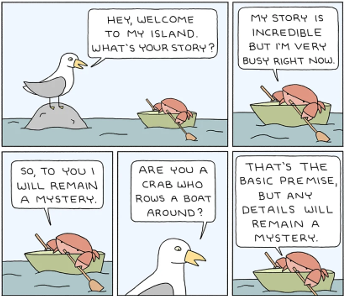
\includegraphics[width=0.5\linewidth]{cp5/classes.png}
    % \end{figure}
\end{center}

\section{Palíndromo}  
Implemente un método recursivo que determine si una cadena de texto es un palíndromo.  

\section{Inversión de Cadena}  
Implemente un método recursivo que invierta una cadena de texto y devuelva el resultado.  

\section{Mínimo Elemento}  
Dado un array que no está necesariamente ordenado, implemente el método que busca recursivamente el menor de los elementos.


\section{Cantidad de elementos}
Implemente un método recursivo que cuente la cantidad de elementos en un arreglo de enteros.
\subsection*{Ejemplo}
Entrada: \([1, 2, 3, 4, 5]\)

Salida: \( 5 \)

\section{Buscar en un arreglo}
Implemente un método recursivo que determine si un número \( x \) está presente en un arreglo de enteros.
\subsection*{Ejemplo}
Entrada: \(a = [1, 2, 3, 4, 5]\), \( x = 3 \)

Salida: \textcolor{blue}{true}

\section{Suma de Elementos}  
Implemente un método recursivo que sume todos los elementos de un arreglo de enteros.  

\section{Suma de Elementos en Matriz}  
Implemente un método recursivo que sume todos los elementos de una matriz de enteros.

\section{Multiplicación}  
Implemente un método recursivo para multiplicar dos números enteros sin utilizar el operador \texttt{*}. Su implementación debe minimizar el número de llamadas recursivas.  

\section{Cantidad de Caminos}  
Implemente el método que devuelva la cantidad de caminos que se pueden tomar para llegar desde la posición (0, 0) hasta la posición ($x$,$x$).

Un camino es una secuencia de puntos con coordenadas enteras que cumple las siguientes condiciones:

\begin{itemize}
    \item \textbf{Distancia:} La distancia entre dos puntos consecutivos en el camino es exactamente una unidad.
    \item \textbf{Secuencia no decreciente:} Las coordenadas \(x\) y \(y\) deben seguir una secuencia no decreciente a lo largo del camino, es decir, en cada paso las coordenadas no pueden disminuir.
    \item \textbf{Restricción de la diagonal:} En ningún momento del camino se debe permitir que \(y\) sea mayor que \(x\), garantizando que siempre se esté debajo o en la misma línea de la diagonal \(y = x\).
\end{itemize}

\subsection*{Ejemplo}
Para llegar a la posición \((3, 3)\), existen exactamente \textbf{5 caminos válidos} que respetan la restricción de la diagonal:

\begin{itemize}
    \item \((0, 0) \to (1, 0) \to (2, 0) \to (3, 0) \to (3, 1) \to (3, 2) \to (3, 3)\),
    \item \((0, 0) \to (1, 0) \to (2, 0) \to (2, 1) \to (3, 1) \to (3, 2) \to (3, 3)\),
    \item \((0, 0) \to (1, 0) \to (1, 1) \to (2, 1) \to (3, 1) \to (3, 2) \to (3, 3)\),
    \item \((0, 0) \to (1, 0) \to (2, 0) \to (2, 1) \to (2, 2) \to (3, 2) \to (3, 3)\),
    \item \((0, 0) \to (1, 0) \to (1, 1) \to (2, 1) \to (2, 2) \to (3, 2) \to (3, 3)\).
\end{itemize}  

\section{Conteo de Pasos en una Escalera}
Implemente un método recursivo que calcule de cuántas maneras distintas se puede subir una escalera de \( n \) peldaños, si se puede avanzar 1, 2 o 3 peldaños a la vez.  

\subsection*{Ejemplo}
Para una escalera de \( 4 \) peldaños, las combinaciones son:

\[
1+1+1+1,\ 1+1+2,\ 1+2+1,\ 2+1+1,\ 2+2,\ 1+3,\ 3+1
\]

El resultado debe ser \( 7 \).

\section{Conjunto de Wirth}  
 El conjunto de Wirth (W) se define como:

\[ 1 \in W \]
\[ \text{Si } x \in W \Rightarrow \{ 2x + 1 \in W, 3x + 1 \in W \} \]

Implemente un método que determine si el número \( x \) pertenece al conjunto de Wirth.
  

\section{Dígitos Crecientes}  
Implemente un método que reciba un entero \( n \) y genere todos los números decimales de \( n \) dígitos cuyos dígitos sean estrictamente crecientes. 

\subsection*{Ejemplo}
Para \( n = 2 \) debe imprimir:  
\begin{equation}
    \begin{aligned}  
    12 \\ 
    13 \\ 
    14 \\ 
    \ldots \\ 
    78 \\
    79 \\
    89  
    \end{aligned}
\end{equation}



\section{Problema del círculo de ejecución}  
Hay $N$ personas en un círculo esperando ser ejecutadas. El conteo comienza en un punto del círculo y sigue una dirección fija. En cada paso, se omiten a ciertas personas y la siguiente persona es ejecutada. La eliminación continúa alrededor del círculo (que va disminuyendo a medida que se eliminan personas) hasta que solo queda una persona, quien es liberada.

Dado el número total de personas $N$ y un número $k$, que indica que se omiten $k-1$ personas y la $k$-ésima persona es ejecutada, la tarea es elegir la persona que sobrevive en el círculo inicial.

\subsection*{Ejemplos:}
\begin{itemize}
    \item \textbf{Entrada:} $N$ = 5 y $k$ = 2\\
        \textbf{Salida:} 3\\
        \textbf{Explicación:} Primero se ejecuta a la persona en la posición 2, luego a la persona en la posición 4, después a la persona en la posición 1, y finalmente a la persona en la posición 5. La persona en la posición 3 sobrevive.
    \item \textbf{Entrada:} $N$ = 7 y $k$ = 3\\
        \textbf{Salida:} 4\\
        \textbf{Explicación:} Las personas en las posiciones 3, 6, 2, 7, 5 y 1 son ejecutadas en ese orden, y la persona en la posición 4 sobrevive.
\end{itemize}

\section{Suma Decreciente}  
Implemente un método que reciba un entero \( n \) y muestre todas las secuencias distintas de enteros positivos que suman \( n \). Por ejemplo, para \( n = 4 \):  
\begin{equation}
    \begin{aligned}
    4 \\ 
    3+1 \\ 
    2+2 \\ 
    2+1+1 \\ 
    1+1+1+1   
    \end{aligned}
\end{equation}

\section{Suma Creciente}  
Implemente un método que reciba un entero \( n \) y muestre todas las secuencias crecientes de enteros positivos que suman \( n \). Por ejemplo, para \( n = 4 \):  
\begin{equation}
    \begin{aligned}
    1+1+1+1 \\
    1+1+2 \\
    1+3 \\
    4
    \end{aligned}
\end{equation}

\section{Búsqueda Binaria}  
Dado un array ordenado de enteros, implemente el método
\texttt{bool BinarySearch(int[] array, int x)}
que realiza una búsqueda binaria recursiva en el array.
  

% \section{Subsecuencia Común Más Larga}
% Implemente un método recursivo que calcule la longitud de la \textbf{subsecuencia común más larga} (LCS, por sus siglas en inglés) entre dos cadenas de texto dadas.

% Una subsecuencia es una secuencia derivada de otra secuencia, eliminando algunos o ningún elemento, pero manteniendo el orden relativo de los elementos restantes. A diferencia de una subcadena, que requiere que los elementos sean contiguos, en una subsecuencia los caracteres pueden no ser adyacentes pero deben aparecer en el mismo orden.

% \subsection*{Ejemplo:}
% Para las cadenas \texttt{''ABCBDBB''} y \texttt{''BDCAB''}, la subsecuencia común más larga es \texttt{''BCB''} y tiene una longitud de 3.

% \section{Inserciones para Palíndromo}  
% Implemente un método que calcule el número mínimo de inserciones necesarias para convertir una cadena en un palíndromo.  

% \section{Distancia entre Strings}  
% Implemente un método recursivo que calcule la distancia entre dos cadenas de texto. Esta distancia se define como el número mínimo de operaciones (inserciones, eliminaciones o sustituciones) necesarias para convertir una cadena en la otra.  

% \section{Recorrido del Caballo}  
% Se desea determinar si es posible recorrer un tablero de ajedrez de \(n \times n\) celdas utilizando un caballo, de manera que, comenzando en la celda superior izquierda (0, 0), el caballo pase exactamente una vez por cada celda. Recuerde que el movimiento del caballo consiste en desplazarse dos celdas en una dirección (horizontal o vertical) y luego una celda en una dirección ortogonal.

\begin{enumerate}[label=\alph*)]
    \item Implemente un método que devuelva si existe al menos un recorrido posible del caballo en un tablero de \(n \times n\).

    \item Implemente un método que devuelva la cantidad total de recorridos posibles que el caballo puede realizar en dicho tablero.
\end{enumerate}


% \section{Máximo y Mínimo}  
% Implemente un método que, dado un arreglo de enteros \(a\), encuentre el valor máximo y el mínimo utilizando \(\frac{3n}{2}\) comparaciones o menos.  

\end{document}
